\documentclass[hidelinks]{article}
\usepackage[utf8]{inputenc}
\usepackage[T1]{fontenc}
\usepackage[margin=1in]{geometry}
\usepackage{graphicx,hyperref,lipsum,multicol}
\title{Analyzing Movies Using Phrase Mining}
\author{Daniel Lee \and Huilai Miao \and Yuxuan Fan}

\begin{document}
\maketitle

\begin{abstract}
\end{abstract}

\begin{multicols}{2}
\section{Introduction}
Movies often capture human culture and major events throughout time. We can retrieve these expressions of human culture and events through a comprehensive textual analysis of movie plots. Here, we propose an analysis of movie plots through the use of phrase mining to extract key phrases that correspond to discrete entities of human culture and events. Such an analysis can help us better understand change of popular topics, public attitudes, major themes, and how overall human culture has progressed throughout history. This analysis is novel since we extract history from movies, an unconventional source, instead of relying on historical texts directly; we expect such a study to provide a unique perspective as a result. In addition, we expect such a study to be especially useful for history non-experts, as we extract key phrases which can provide relevant and insightful keywords for further research by the reader. We perform this analysis on a large dataset of movie plot summaries from English movies over the past century.

Previous work addresses either a comprehensive analysis of movie history or the use of phrase mining for natural language processing, but not both. Previous analyses of movies are limited since they tend to use extract words or phrases via the use of raw frequencies instead of a sophisticated phrase mining technique such as AutoPhrase \cite{DBLP:journals/corr/ShangLJRVH17}. Here, we explore a novel approach to apply phrase mining to the analysis of movies.

\section{Data}
Our dataset comes from the \href{http://www.cs.cmu.edu/~ark/personas/}{CMU Movie Summary Corpus} \cite{Bamman2013LearningLP}.
\end{multicols}

\begin{figure}[h]
\centering
\caption{Number of movies in the dataset}
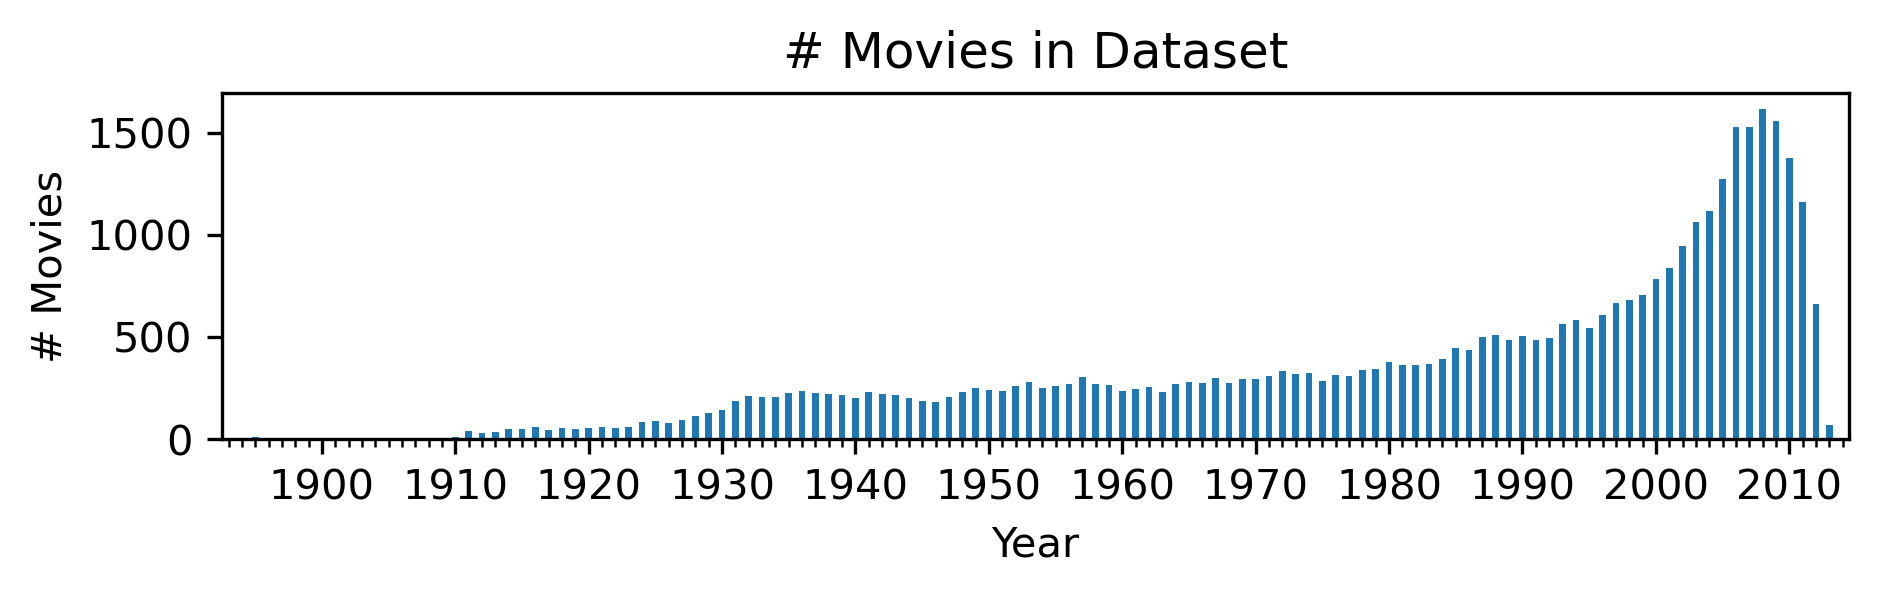
\includegraphics[width=5in]{figures/number_movies_per_year_bar_chart.png}
\end{figure}
\begin{multicols}{2}

\section{Methods}
\subsection{EDA}
\subsection{Classification}
\subsection{Clustering}

\section{Results}
\subsection{EDA}
\subsection{Classification}
\subsection{Clustering}

\section{Discussion}
\end{multicols}

\nocite{10.1145/2723372.2751523}
\bibliographystyle{plain}
\bibliography{report}

\section{Appendix}

\end{document}
